\documentclass[a4paper]{article}

%% Language and font encodings
\usepackage[french]{babel}
\usepackage[utf8x]{inputenc}
\usepackage[T1]{fontenc}

%% Sets page size and margins
\usepackage[a4paper,top=3cm,bottom=2cm,left=3cm,right=3cm,marginparwidth=1.75cm]{geometry}
\usepackage{mathtools, bm}
\usepackage{amssymb, bm}

\renewcommand{\thesection}{\arabic{section})}
\renewcommand{\thesubsection}{\alph{subsection})}


%% Useful packages
\usepackage{amsmath}
\usepackage{graphicx}
\usepackage[colorinlistoftodos]{todonotes}
\usepackage[colorlinks=true, allcolors=black]{hyperref}

\usepackage{algorithm2e}
\usepackage[section]{placeins}

\title{
    \begin{minipage}\linewidth
        \centering\bfseries\sffamily
        Méthodes et Programmation Numériques Avancées
        \vskip10pt
        \large TP1
         \vskip10pt
         \large Produit Scalaire - Produit Matrice Vecteur - Gram-Schmidt
    \end{minipage}}
\author{Maxime Kermarquer - M2 CHPS}
\date{}

\begin{document}
\maketitle

\vskip 1cm
\hrule
\medskip
  \tableofcontents
\medskip
\hrule
\vskip 1.5cm

\section*{Introduction}
Afin de nous familiariser avec les méthodes numériques, il nous a été demandé d'étudier et d'implémenter le produit scalaire, le Produit Matrice Vecteur et l'algorithme de Gram-Schmidt.

Nous allons présenter une analyse des complexités de ces différents problèmes en séquentiel mais aussi en parallèle. Nous présenterons les courbes de performances obtenues, ainsi que nos observations sur celle ci.

Dans ce rapport, nous commencerons par présenter les travaux réalisés sur le produit scalaire, puis nous détaillerons le Produit Matrice Vecteur et la dernière partie sera consacrée à l'algorithme de Gram-Schmidt.

\newpage


\part{Produit scalaire}

\section{Cas séquentiel}

%\subsection{Pseudo Code}
%\subsection{Complexité}


La méthode utilisée pour réaliser le produit scalaire séquentielle est décrite dans la figure \ref{fig:algo_ps}.

\begin{figure}[h]
\fbox{
	\begin{algorithm}[H]
    	\SetKwInOut{Input}{input}\SetKwInOut{Output}{output}
        
    	\Input{$\overrightarrow{a}$ et $\overrightarrow{b}$ deux vecteurs de taille $n$}
        \Output{$resultat$ le produit scalaire de $\overrightarrow{a}$ et $\overrightarrow{b}$}
        \vskip 5pt
        $resultat \leftarrow 0$
        \vskip 5pt
    	\For{$i\leftarrow 0$ \KwTo $n$}{
        	$tmp$ $\leftarrow$ $a_{i} * b_{i}$ \;
            $resultat$ $\leftarrow$ $resultat + tmp$ \;
        }
        \vskip 5pt
        \Return $resultat$
	\end{algorithm}
}
	\caption{L'algorithme du produit scalaire en séquentiel}%	
	\label{fig:algo_ps}%
\end{figure}

On peut calculer la complexité en temps de la méthode, on a :
\begin{itemize}
\item $n$ multiplications
\item $n$ additions	
\end{itemize}
Ce qui nous fait une complexité en temps de : \textbf{$\mathcal{O}(2n)$} \\
Pour la complexité en espace, on a deux vecteurs de taille $n$ : \textbf{$\mathcal{O}(2n)$}


\section{Cas parallèle}

La méthode utilisée pour réaliser le produit scalaire en parallèle est décrite dans la figure \ref{fig:algo_ps_parallele}.

\begin{figure}[h]
\fbox{
	\begin{algorithm}[H]
    	\SetKwInOut{Input}{input}\SetKwInOut{Output}{output}
        \SetKwFunction{Reduction}{Reduction}
        
        Pour $p$ processus\\
    	\Input{$\overrightarrow{a}$ et $\overrightarrow{b}$ deux vecteurs de taille $n$}
        \Output{$resultat$ le produit scalaire de $\overrightarrow{a}$ et $\overrightarrow{b}$}
        \vskip 5pt
        $resultat \leftarrow 0$ \;
        $resultat.processus \leftarrow 0$ \;
        $k \leftarrow \frac{n}{p}$ \;
        \vskip 5pt
    	\For{$i\leftarrow 0$ \KwTo $k$}{
        	$tmp$ $\leftarrow$ $a_{i} * b_{i}$ \;
            $resultat.processus \leftarrow resultat.processus + tmp$ 
        }
        \Reduction{$resultat.processus$, ADDITION, $resultat$}\;
        \vskip 5pt
        \Return $resultat$
	\end{algorithm}
}
	\caption{L'algorithme du produit scalaire en parallèle}%	
	\label{fig:algo_ps_parallele}%
\end{figure}

Le nombre d'opérations sera divisé par les $p$ processus on a donc un complexité en temps est de : \textbf{$\mathcal{O}(2n / p)$} \\
Pour la complexité en espace, on a toujours : \textbf{$\mathcal{O}(2n)$}

\section{Résultat obtenus}

Les tests ont étaient réalisés sur une machine à quatre cœurs. On a fait varier la taille des vecteurs afin d'étudier le temps d'exécution du produit scalaire. Les résultats sont présentés dans la figure \ref{fig:courbe_ps}.

\begin{figure}[h!]
	\begin{center}
		\includegraphics[scale=0.80]{Courbes/produit_scal_temps_taille.eps}
	\end{center}
	\caption{Évolution du temps de calcul du produit scalaire en fonction de la taille des vecteurs}
	\label{fig:courbe_ps}
\end{figure}

\FloatBarrier

Les deux courbes ont une croissance linéaire. La courbe parallèle a néanmoins une croissance plus faible. On observe que la méthode séquentielle est plus efficace pour les petites tailles de vecteurs comme on peut le voir dans la figure \ref{fig:courbe_ps2}.
Le coût du parallélisme est alors plus important que son gain. Le parallélisme devient intéressant pour des produits scalaire de taille supérieur à environ 1100.

\begin{figure}[h]
	\begin{center}
		\includegraphics[scale=0.80]{Courbes/produit_scal_croisement.eps}
	\end{center}
   	\caption{Évolution du temps de calcul du produit scalaire en fonction de la taille des vecteurs}
	\label{fig:courbe_ps2}
\end{figure}

\FloatBarrier

\part{Produit Matrice Vecteur}

\section{Cas séquentiel}

La méthode utilisée pour réaliser le Produit Matrice Vecteur séquentiellement est décrite dans la figure \ref{fig:algo_pmv}. \\

\begin{figure}[h]
\fbox{
	\begin{algorithm}[H]
    	\SetKwInOut{Input}{input}\SetKwInOut{Output}{output}
        
    	\Input{$A$ une matrice de taille  $m \times n$ et $\overrightarrow{v}$ un vecteur de taille $n$}
        \Output{$\overrightarrow{r}$ le vecteur résultant du Produit Matrice Vecteur de $A$ et $\overrightarrow{v}$ de taille $m$}
        \vskip 5pt

    	\For{$i\leftarrow 0$ \KwTo $m$}{
        	$r_{i}$ $\leftarrow$ $\langle A[i], v\rangle$ \;
        }
        \vskip 5pt
        \Return $\overrightarrow{r}$
	\end{algorithm}
}
	\caption{L'algorithme du Produit Matrice Vecteur séquentiel}%	
	\label{fig:algo_pmv}%
\end{figure}


On réalise $m$ produit scalaire, on a donc une complexité de : \textbf{$\mathcal{O}(2mn)$}. Lorsque $m \rightarrow n$ : \textbf{$\mathcal{O}(n^2)$}.
Pour la complexité en espace, on a :
\begin{itemize}
\item Une matrice de $m \times n$
\item Un vecteur de taille $n$
\item Un vecteur de taille $m$
\end{itemize}
Ce qui nous fait une complexité en espace de : \textbf{$\mathcal{O}(mn + m + n)$}.

\section{Cas parallèle}


La méthode utilisée pour réaliser le Produit Matrice Vecteur en parallèle est décrite dans la figure \ref{fig:algo_pmv_par}. \\

\begin{figure}[h]
	\fbox{
      \begin{algorithm}[H]
          \SetKwInOut{Input}{input}\SetKwInOut{Output}{output}
          \SetKwFunction{Regroupement}{Regroupement}
          \SetKwComment{Comment}{}{}

          Pour $p$ processus\\
          \Input{$A$ une matrice de taille  $m \times n$ et $\overrightarrow{v}$ un vecteur de taille $n$}
          \Output{$\overrightarrow{r}$ le vecteur résultant du Produit Matrice Vecteur de $A$ et $\overrightarrow{v}$ de taille $m$}
          \vskip 5pt

          $k \leftarrow \frac{m}{p}$ \; \vskip 5pt
          \Comment{r.processus est de taille k}
          $\overrightarrow{r.processus} $\; \vskip 5pt 

          \For{$i\leftarrow 0$ \KwTo $k$}{
              $r.processus_{i}$ $\leftarrow$ $\langle A[i], v\rangle$ \;
          }

          \vskip 5pt
          \Comment{Regroupement des $\overrightarrow{r.processus}$ dans $\overrightarrow{r}$} 
         \Regroupement{$resultat.processus$, $r$}\;

          \vskip 5pt
          \Return $\overrightarrow{r}$
      \end{algorithm}
    }
	\caption{L'algorithme du Produit Matrice Vecteur en parallèle}%	
	\label{fig:algo_pmv_par}%
\end{figure}


Comme pour le produit scalaire, la complexité en temps du Produit Matrice Vecteur sera divisé par $p$, auquel on ajoute un coût de parallélisation $C$: \textbf{$\mathcal{O}(\frac{n^2}{p} + C)$}.\\
La complexité en espace reste la même : \textbf{$\mathcal{O}(mn + m + n)$}.



\section{Résultat obtenus}

Comme pour le produit scalaire, on a fait varier la taille du vecteur et de la matrice afin d'étudier le temps d'exécution du Produit Matrice Vecteur. Les résultats sont présentés dans la figure \ref{fig:courbe_pmv}.

\begin{figure}[h]
	\begin{center}
		\includegraphics[scale=0.80]{Courbes/pmv_temps_taille.eps}
	\end{center}
   	\caption{Évolution du temps de calcul Produit Matrice Vecteur en fonction de la taille des données}
	\label{fig:courbe_pmv}
\end{figure}

\FloatBarrier

Bien que l'échantillon de test est assez petit, les courbes ont l'air d'avoir des croissances exponentielles. Ce qui correspond aux complexités théoriques décrites précédemment.

\part{Gram-Schmidt}

Nous nous sommes ensuite concentrés sur l'algorithme de Gram-Schmidt et sa version modifiée.

\section{Description de la méthode}

L'algorithme va réaliser une orthonormalisation d'un ensemble de vecteurs.
% qui se décompose donc en deux étapes :
% \begin{enumerate}
% \item Une projection orthogonale
% \item Une normalisation
% \end{enumerate}
La version modifiée permet de corriger les erreurs d'arrondis de la version classique. Les détails de ces algorithmes sont donné dans la figure \ref{fig:algo_gs}.

\begin{figure}
	\begin{center}
    $A \in \mathbb{R}^{m \times n}$ avec $m \geq n$, et $A$ a $n$ colonnes linéairement indépendantes $a_{1}, a_{2}, \cdots, a_{n}$.
    \vskip 0.5cm
    \begin{minipage}[l]{0.35\linewidth}
    \fbox{
      \begin{algorithm}[H]
      	\textbf{Classique}\\
          \For{$k\leftarrow 1$ \KwTo $n$}{
          	$w \leftarrow a_{k}$ \\
            \For{$j\leftarrow 1$ \KwTo $k-1$}{
				$r_{jk} \leftarrow q_{j}^{t}w$
            }
            \For{$j\leftarrow 1$ \KwTo $k-1$}{
				$w \leftarrow w - r_{jk}q_{j}$
            }
            $r_{kk} \leftarrow ||w||_{2}$ \\
            $q_{k} \leftarrow \frac{w}{r_{kk}}$ \\
          
          }
      \end{algorithm}
      }
      \end{minipage}
      \hspace{1cm}
      \begin{minipage}[c]{0.35\linewidth}
      \fbox{
      \begin{algorithm}[H]
      	\textbf{Modifié}\\
          \For{$k\leftarrow 1$ \KwTo $n$}{
          	$w \leftarrow a_{k}$ \\
            \For{$j\leftarrow 1$ \KwTo $k-1$}{
				$r_{jk} \leftarrow q_{j}^{t}w$ \\
				$w \leftarrow w - r_{jk}q_{j}$ \\
            }
            $r_{kk} \leftarrow ||w||_{2}$ \\
            $q_{k} \leftarrow \frac{w}{r_{kk}}$ \\
          
          }
      \end{algorithm}
      }
      \end{minipage}
      \end{center}
      \caption{Algorithme de Gram-Schmidt classique et modifié}
      \label{fig:algo_gs}
\end{figure}


\section{Résultats obtenus}

On a augmenter le nombre de vecteurs à orthonormaliser, afin d'observer le comportement des deux version de l'algorithme. Nous pouvons ainsi étudier l'erreur de précision de chacun.

\begin{figure}[h]
	\begin{center}
		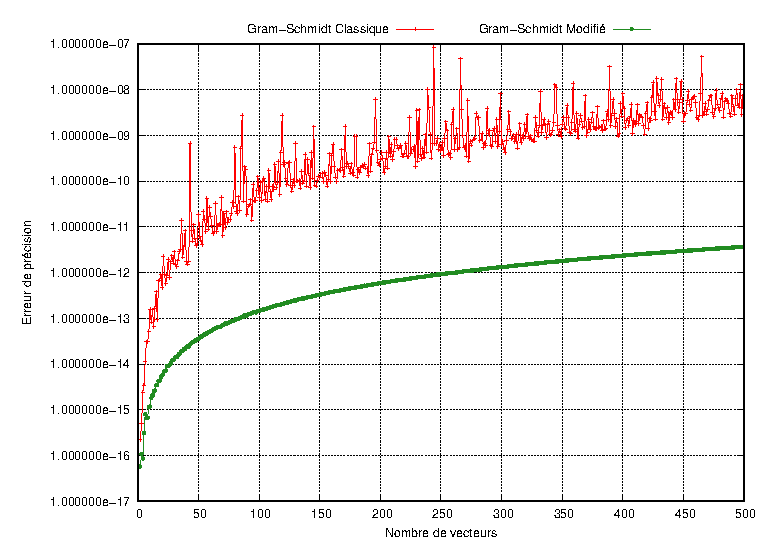
\includegraphics[scale=0.80]{Courbes/gram_schmidt.eps}
	\end{center}
    \caption{Évolution de l'erreur de précision en fonction de la taille des données}
	\label{fig:courbe_gs}
\end{figure}

\FloatBarrier

On observe que l'erreur est croissante. La version classique a de nombreux pics dans sa progression, alors que la courbe de la version modifiée est régulière. La version modifiée offre une meilleure précision.


\section*{Conclusion}
Dans ce premier TP, nous avons été initier aux méthodes numériques, et comment les adapter pour des architectures parallèles. Nous avons étudier leurs complexités en temps, espace et précision. Avec Gram-Schmidt, nous avons pus voir que certaines optimisations anodines permettent un réel gain de complexité. 

L'apprentissage de cette approche, des métriques de performances nous sera utile pour les prochaines études des méthodes itératives.



\end{document}